\documentclass[tikz,border=5pt]{standalone}
\usepackage{luatexja}
\usepackage[hiragino-pron]{luatexja-preset}
\usepackage{amsmath,amssymb}
\usepackage{pgfplots}
\pgfplotsset{compat=1.18}
\usetikzlibrary{arrows.meta,calc,decorations.markings,patterns,positioning}

% Common styles
\tikzset{
  axis/.style={-{Stealth[length=6pt]}, thick},
  curve/.style={thick, red},
  dashed curve/.style={thick, dashed, blue},
  dot/.style={circle, fill, inner sep=1.5pt},
  open dot/.style={circle, draw, fill=white, inner sep=1.5pt},
}

\begin{document}
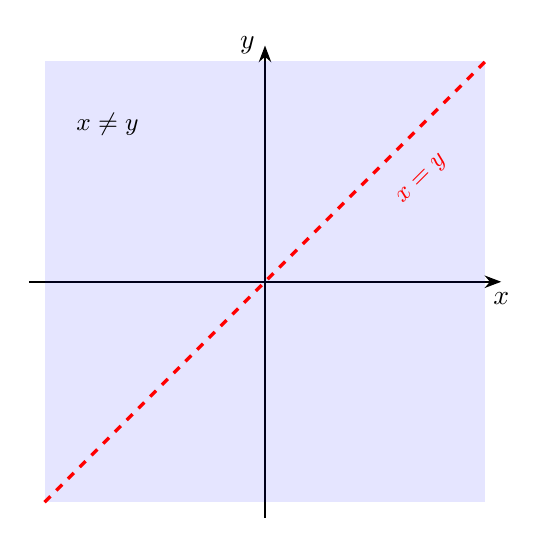
\begin{tikzpicture}
  % Axes
  \draw[axis] (-3,0) -- (3,0) node[below] {$x$};
  \draw[axis] (0,-3) -- (0,3) node[left] {$y$};

  % Fill entire plane with light blue
  \fill[blue, opacity=0.1] (-2.8,-2.8) rectangle (2.8,2.8);

  % Excluded line x=y (hatched / dashed)
  \draw[red, dashed, very thick] (-2.8,-2.8) -- (2.8,2.8);

  % Label
  \node[red, font=\small, rotate=45] at (2,1.3) {$x = y$};
  \node[font=\small] at (-2,2) {$x \neq y$};
\end{tikzpicture}
\end{document}
